\documentclass[paper=a4, pagesize, twoside, openright, draft=false,
BCOR7mm, DIV13, fontsize=11pt, headings=normal, footinclude=false, 
chapterprefix = false, toc=listof, ngerman, parskip=half]{scrartcl} % doppelseitiger Druck

%%%%%%%%%%%%%%%%%%%%%%%%%%%%%%%%%%%%%%%%%%%%%%%%%%%%%%%%%%%%%%%%%%%%%%%%%%%%%%%%%%%%%%%%%
%%%%%%%%%%%%%%%%%%%%%%%%%%%%%%%%%%%%%%%%%%%%%%%%%%%%%%%%%%%%%%%%%%%%%%%%%%%%%%%%%%%%%%%%
\usepackage{D:/Daten/HM/dsvFPGA/Uebungen/HM/dsvFPGA_ueb_style_v3}
%%%%%%%%%%%%%%%%%%%%%%%%%%%%%%%%%%%%%%%%%%%%%%%%%%%%%%%%%%%%%%%%%%%%%%%%%%%%%%%%%%%%%%%%
%
%\includeonly{2010-DSP_FPGA-Ueb_Kap_1_2}
%
\hypersetup{
pdftitle={Asynchronous Sample Rate Conversion},
                   pdfauthor={Christian Muenker},
                   pdfsubject={Asynchronous Sample Rate Conversion},
                   pdfkeywords={SRC, ASRC, Python}
                   }
\def\CodePath{scripts/}
\def\pyFirstLine{31}
\def\mlFirstLine{20}
%
%
\begin{document}
%\renewmdenv[linecolor=red,frametitle={Wichtige Begriffe}]{infobox}

%\frontmatter
%%%%%%%%%%%%%%%%%%%%%%%%%%%%%%%%%%%%%%%%%%%%%%%%%%%%%%%%%%%%%%%%%%%%%%%%%%%%%%%%%%%%%%%%%
%%%%%%%%%%%%%%%%%%%%%%%%%%%%%%%%%%%%%%%%%%%%%%%%%%%%%%%%%%%%%%%%%%%%%%%%%%%%%%%%%%%%%%%%%
\author{Prof. Dr. Christian M�nker}
\title{Asynchronous Sample Rate Conversion}
\date{\today}
%\maketitle
\begin{titlepage}
\begin{center}
\begin{Huge}Asynchronous Sample Rate Conversion\end{Huge}\\[1cm]
\begin{huge}ASRC\end{huge}
\\[1cm]
\LARGE Prof. Dr. Christian M\"unker
\vfill
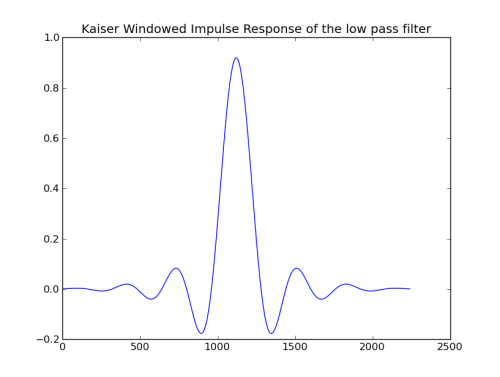
\includegraphics[width=13cm]{img/KaiserIR.png}

\footnotesize{sinc-Funktion}
\vfill
\Large \today \\[1cm]
\href{mailto:Christian.Muenker@hm.edu}{Christian.Muenker@hm.edu}
\end{center}
\end{titlepage}

%
%***********************************************************************%
%*******               TABLE OF CONTENTS                        ********%
%***************                                        ****************%
\clearpage
\phantomsection % needed for correct TOC and hyperlinks
\tableofcontents
\addcontentsline{toc}{section}{Inhaltsverzeichnis}

%
%\def\thesection{\arabic{chapter}.\arabic{section}} 
%\include{DSP_FPGA-Ueb_Changes}
%\addcontentsline{toc}{chapter}{�nderungen}

%\def\thesection{Aufgabe \arabic{chapter}.\arabic{section}} 

%\setcounter{lofdepth}{2} % List of figures mit subfigures


%%%%%%%%%%%%%%%%%%%%%%%%%%%%%%%%%%%%%%%%%%%%%%%%%%%%%%%%%%%%%
\setcounter{topnumber}{3} % max. Anzahl von Gleitobjekten im oberen Teil der Seite

\section{Worum geht's?}

\textbf{ASRC} ist 
Literatur:\\

\begin{description}
\item [JOS] \texttt{Ausf�hrlicher Artikel von Julius O. Smith zu Resampling durch "`Bandbegrenzte Interpolation"'} \url{https://ccrma.stanford.edu/~jos/resample/resample.html}
\item [Uri Nieto] Audio Resampling in Python, \url{http://urinieto.com/2011/05/audio-resampling-in-python/}
\end{description}




%\begin{figure}[ht]
%\centering
%\includegraphics[width = 0.8\textwidth]{ueb-PY-git-local-remote}
%\caption{Grundlegende Git - Operationen [\url{http://www.terminus-notfallmedizin.de/blog/?p=824}]}
%\label{fig:Py-git-local-remote}
%\end{figure}

\begin{infobox}
\begin{description}
\item [Sample Rate] (Abtastrate) die Rate, mit der ein zeitdiskretes Signal vorliegt
\item [Upsampling] Erh�hen der Abstastrate um einen ganzzahligen Faktor, die fehlenden Samples werden durch Null gef�llt (zero-stuffing) oder durch Wiederholen des letzten Werts (Zero-Order Hold). Dabei entstehen Kopien des ehemaligen Basisbands bis zur neuen -> Nyquistfrequenz, sog. -> Images, die durch Anti-Image Filter entfernt werden m�ssen. 
\item [Downsampling] Verringerung der Abtastrate um einen ganzzahligen Faktor durch Weglassen von Abtastwerten. Ohne vorherige Bandbreitenbegrenzung (Anti-Alias Filterung) besteht die Gefahr von -> Aliasing.
\item [Resampling]
\item [Synchron] wenn sich das Verh�ltnis von zwei Abtastraten durch ein einfachen Bruch ausdr�cken l�sst, z.B. beim Resampling von 44.1kHz to 48kHz, 44.1/48 = 147 / 160 .
\item [Asynchron] wenn die zwei Abtastraten kein einfaches rationales Verh�ltnis haben
\end{description}
\end{infobox}

\section{Typische Arbeitsschritte}


\end{document}
